\documentclass[english]{beamer}
%\documentclass[finnish,english,handout]{beamer}

% Uncomment if want to show notes
%\setbeameroption{show notes}

\mode<presentation>
{
  \usetheme{Warsaw}
  % oder ...

  %\setbeamercovered{transparent}
  % oder auch nicht
}


%\usepackage[pdftex]{graphicx}
\usepackage[T1]{fontenc}
\usepackage[latin1]{inputenc}
%\usepackage[T1,mtbold,lucidacal,mtplusscr,subscriptcorrection]{mathtime}
\usepackage{times} % times
\usepackage{amsmath}
\usepackage[varqu,varl]{inconsolata} % typewriter
\usepackage{microtype}
\usepackage{url}
\urlstyle{same}

\hypersetup{%
  bookmarksopen=true,
  bookmarksnumbered=true,
  pdftitle={Use of reference models in model selection},
  pdfsubject={Bayesian model selection},
  pdfauthor={Aki Vehtari},
  pdfkeywords={},
  pdfstartview={FitH -32768},
  colorlinks=true,
  linkcolor=blue,
  citecolor=blue,
  filecolor=blue,
  urlcolor=blue
}

% \definecolor{hutblue}{rgb}{0,0.2549,0.6784}
% \definecolor{midnightblue}{rgb}{0.0977,0.0977,0.4375}
% \definecolor{navyblue}{rgb}{0,0,0.5}
% \definecolor{hutsilver}{rgb}{0.4863,0.4784,0.4784}
% \definecolor{lightgray}{rgb}{0.95,0.95,0.95}
% \definecolor{section}{rgb}{0,0.2549,0.6784}
% \definecolor{list1}{rgb}{0,0.2549,0.6784}
% \renewcommand{\emph}[1]{\textcolor{navyblue}{#1}}

\graphicspath{../luku1}

\pdfinfo{
          /Title      (Bayesian data analysis)
          /Author     (Aki Vehtari) %
          /Keywords   (Bayesian probability theory, Bayesian inference, Bayesian data analysis)
}


\parindent=0pt
\parskip=8pt
\tolerance=9000
\abovedisplayshortskip=0pt

\setbeamertemplate{navigation symbols}{}
\setbeamertemplate{headline}[default]{}
\setbeamertemplate{headline}[text line]{\insertsection}
\setbeamertemplate{footline}[frame number]


\def\o{{\mathbf o}}
\def\t{{\mathbf \theta}}
\def\w{{\mathbf w}}
\def\x{{\mathbf x}}
\def\y{{\mathbf y}}
\def\z{{\mathbf z}}

\DeclareMathOperator{\E}{E}
\DeclareMathOperator{\Var}{Var}
\DeclareMathOperator{\var}{var}
\DeclareMathOperator{\Sd}{Sd}
\DeclareMathOperator{\sd}{sd}
\DeclareMathOperator{\Bin}{Bin}
\DeclareMathOperator{\Beta}{Beta}
\DeclareMathOperator{\logit}{logit}
\DeclareMathOperator{\N}{N}
\DeclareMathOperator{\U}{U}
\DeclareMathOperator{\BF}{BF}
%\DeclareMathOperator{\Pr}{Pr}
\def\euro{{\footnotesize \EUR\, }}
\DeclareMathOperator{\rep}{\mathrm{rep}}


\title[]{Bayesian data analysis}
\subtitle{Practical matters}

\author{Aki Vehtari}

\institute[Aalto University]{}

\begin{document}

\section{Course contents}


\begin{frame}
  \frametitle{Bayesian data analysis (Aalto fall 2020)}  %
  \framesubtitle{}
  \begin{itemize}
  \item Book: Gelman, Carlin, Stern, Dunson, Vehtari \& Rubin: Bayesian Data
    Analysis, Third Edition. {\footnotesize (online pdf available)}
  \item The course website has more detailed information than these slides\\
    {\small\url{https://avehtari.github.io/BDA_course_Aalto/Aalto2020.html}}
  \item Timetable: see the course website
    \item TAs: Alejandro Catalina, Akash Dhaka, Kunal Ghosh, Noa
      Kallioinen, Anton Mallasto, Topi Paananen, Teemu S�ilynoja
    % \item Oodi mentions TA session this week on Wednesday, but that
    %   has cancelled.
    \end{itemize}
    \vspace{-\baselineskip}
 \begin{center}
   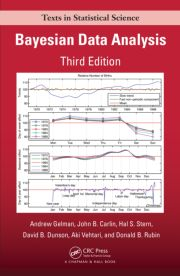
\includegraphics[width=2.6cm]{figs/BDA3.jpg}
 \end{center}

\end{frame}

\begin{frame}{Stan}
  \frametitle{Zoom webinar}  %

  \begin{itemize}
  \item TAs as ``Panelists''
  \item Chat
  \item Q\&A
  \item Polls
  \item Raising hand
  \end{itemize}
  
\end{frame}

\begin{frame}
  \frametitle{Bayesian data analysis}  %
  \framesubtitle{Pre-requisites}
  \begin{itemize}
  \item Basic terms of probability theory
    \begin{itemize}
    \item probability, probability density, distribution
    \item sum, product rule, and Bayes' rule
    \item expectation, mean, variance, median
    \end{itemize}
  \item Some algebra and calculus
  \item Basic visualisation techniques (R or Python)
    \begin{itemize}
    \item histogram, density plot, scatter plot
    \end{itemize}
  \end{itemize}

  These will be tested with the first assignment round

\end{frame}

\begin{frame}
  \frametitle{Bayesian data analysis}  %
  \framesubtitle{Pre-requisites}
  \begin{itemize}
  \item What to do if the course seems to be too difficult
    \begin{itemize}
    \item refresh your memory on pre-requisites
    \item ask for help
    \item consider reading Regression and Other Stories \url{https://avehtari.github.io/ROS-Examples/}
    \item consider reading Statistical rethinking + watching videos \url{https://xcelab.net/rm/statistical-rethinking/}
    \end{itemize}
  \end{itemize}

\end{frame}


\begin{frame}
  \frametitle{Bayesian data analysis}  %
  \framesubtitle{Learning styles}

  \begin{itemize}
  \item Reading
  \item Listening lectures
  \item Solving problems
    \begin{itemize}
    \item mathematical derivations
    \item programming
    \end{itemize}
  \end{itemize}
  
\end{frame}

% \begin{frame}
%   \frametitle{Bayesian data analysis}  %
%   \framesubtitle{Course contents}
%   \begin{itemize}
%   \item Background (Ch 1)
%   \item Single-parameter models (Ch 2)
%   \item Multiparameter models (Ch 3)
%   \item Computational methods (Ch 10)
%   \item Markov chain Monte Carlo (Ch 11--12)
%   \item Stan and probabilistic programming
%   \item Hierarchical models (Ch 5)
%   \item Model checking (Ch 6)
%   \item Evaluating and comparing models (Ch 7)
%   \item Decision analysis (Ch 9)
%   \item Large sample properties and Laplace approximation (Ch 4)
%   \item In addition you learn workflow for Bayesian data analysis
%   \end{itemize}
  
% \end{frame}

\begin{frame}
  \frametitle{Bayesian data analysis}  %
  \framesubtitle{Example analyses}
  \begin{itemize}
  \item Treatment/control
    \begin{itemize}
    \item randomize patients to treatment or control
    \item is the treatment effective?
    \end{itemize}
    \pause
  \item Continuous valued treatment
    \begin{itemize}
    \item randomize patients with different dosages
    \item which dosage is sufficient without too many side effects?
    \end{itemize}
    \pause
  \item Different effects for different patients?
    \begin{itemize}
    \item Is the treatment effect different for male/female, child/adult, light/heavy, ...
    \end{itemize}
  \end{itemize}

\end{frame}

\begin{frame}
  \frametitle{Bayesian data analysis}  %
  \framesubtitle{Computer exercises}
  \begin{itemize}
  \item Basic visualisation techniques
  \item Binomial distribution -- Algae
  \item Normal distribution -- Windshield
  \item Difference between binomials -- Treatment/control
  \item Difference between normals -- Windshield
  \item Generalized linear model (GLM) + importance sampling -- Bioassay
  \item GLM + Metropolis + convergence diagnostics -- Bioassay
  \item GLM + Bioassay + Stan
  \item Linear model + Stan
  \item Hierarchical model + Stan
  \item Model seletion + Stan
  \end{itemize}

\end{frame}

\begin{frame}{Stan}
  
  Stan is a probabilistic programming framework and ecosystem

  40+ developers, 100+ contributors, 100K+ users

  R, Python, Julia, Scala, Stata, Matlab, command line interfaces
  
  More than 100 R packages using Stan
  
  % 
\includegraphics[width=2cm]{Stan_logo.png}
  \center
  \vspace{\baselineskip}
  
\includegraphics[width=2.5cm]{stan_logo_wide.png}\\
  mc-stan.org
% \includegraphics[width=11cm]{mystery.jpeg}

\end{frame}

\begin{frame}
  \frametitle{Bayesian data analysis}  %
  \framesubtitle{Assessment}
  \begin{itemize}
  \item Exercises 2/3, and project work and presentation 1/3
     \begin{itemize}
     \item Minimum of 50\% of points must be obtained from both the project work and the exercises.
     % \item Preliminary grade boundaries\\
     %   <50\%=0, 50\%-60\%=1, 60\%-70\%=2, 70\%-80\%=3, 80\%-90\%=4, >90\%=5
     \end{itemize}
  \end{itemize}

\end{frame}

\begin{frame}
  \frametitle{Bayesian data analysis}  %

  \begin{itemize}
  \item Pre-recorded lectures describe basics and give broader overview
    \begin{itemize}
    \item written material has all the details and self-study
      is possible
    \end{itemize}
  \item Supporting material and assignments in
    {\small\url{https://avehtari.github.io/BDA_course_Aalto/Aalto2020.html}}
    \begin{itemize}
    \item reading instructions and chapter notes
    \item demos
    \item slides (not very useful without the videos)
    \item video clips
    \item links to additional material
    \end{itemize}
   \item R demos {\small\url{https://avehtari.github.io/BDA_course_Aalto/demos.html\#BDA_R_demos}}
  \item (Python demos {\small\url{https://avehtari.github.io/BDA_course_Aalto/demos.html\#BDA_Python_demos})}
  \item Aalto chat instance
  \end{itemize}

\end{frame}

\begin{frame}
  \frametitle{Bayesian data analysis}  %
  \framesubtitle{Exercises}
  \begin{itemize}
  \item Weekly exercises (some have two week time)
    \begin{itemize}
    \item R (Python) simulation exercises
    \item Stan probabilistic programming exercises (via R (Python))
    \end{itemize}
  \item Related R (Python) demos available
  \item TAs available: see Oodi for exercise sessions
  \item Exercise deadlines on Sunday (see detailed info in the course web page)
  \item After exercise deadline grading period Monday--Tuesday
  \item Students grade 3 other exercises using peergrade.io
  \end{itemize}
  
\end{frame}

\begin{frame}
  \frametitle{Bayesian data analysis}  %
  \framesubtitle{R vs Python}

  \begin{itemize}
  \item We strongly recommend using R in the course as there are more
    packages for Stan and statistical analysis in general in R
  \item If you are already fluent in Python, but not in R, then using Python
    may be easier, but it can still be more useful to learn also R
  \end{itemize}
  
\end{frame}

\begin{frame}
  \frametitle{Bayesian data analysis}  %
  \framesubtitle{Exercises}
  \begin{itemize}
  \item Exercises are given on PeerGrade (also available in the course website)
  \item Exercises are returned and graded on Peergrade
  \end{itemize}
\end{frame}

\begin{frame}
  \frametitle{Exercises}  %
  \framesubtitle{peergrade.io}
  \begin{itemize}
  \item Used in BDA course since 2016
  \item Each student grades 3 exercises (randomly distributed)
  \item Detailed grading instructions -- rubric (available also on the course website)
  \item Also text feedback
  \item Possible to flag inappropriate grading
  \item TAs check flagged gradings
  \item Possible to give thumb up for great feedback
    \begin{itemize}
    \item those who give good feedback will get bonus points
    \end{itemize}
  \end{itemize}
  
\end{frame}

\begin{frame}
  \frametitle{Exercises}  %
  \framesubtitle{peergrade.io}

  \begin{itemize}
  \item Combined score: 70\% submission performance, 30\% feedback performance
    \pause
  \item Hand-in score:
    \begin{itemize}
    \item averaging the scores from peers
    \item after flagging teacher may overrule the score
    \item different exercises have different weight
    \end{itemize}
    See details at \url{http://help.peergrade.io/interfaces-and-features/grading-and-scores/the-hand-in-score}
    \pause
  \item Feedback score:
    \begin{itemize}
    \item When students receive a review, they are asked to react to
      it using a scale ranging from "Not useful at all" to "Extremely
      useful".
    \item These ratings each correspond to a score between 0\% and 100\%.
    \item The feedback score is the average of the reaction scores.
    \end{itemize}
    
  \end{itemize}
  
\end{frame}

\begin{frame}
  \frametitle{Peergrade.io}  %
  \framesubtitle{Registration}
  \begin{itemize}
  \item Go to peergrade.io/join
  \item Use class code: (see MyCourses announcements)
  \item Use your Aalto email or we can't match you to your student id
    % \begin{itemize}
    % \item Aalto is getting campus license and integration to Oodi, but
    %   lawyers are still checking data protection issues
    % \end{itemize}
  \end{itemize}
  
\end{frame}

\begin{frame}
  \frametitle{Project work}  %
  \framesubtitle{}
  \begin{itemize}
  \item Project work in groups of 1--3
    \begin{itemize}
    \item combines all the pieces learned in one project work
    \item R or Python notebook report
    \item project report peer graded
    \item oral presentation graded by me and TAs
    \end{itemize}
  \end{itemize}
  
\end{frame}

\begin{frame}

  
\end{frame}  

\end{document}

%%% Local Variables:
%%% mode: latex
%%% TeX-master: t
%%% End:
